\chapter{Кратность, энтропия и равновесие при ограничениях}

\lectureoverview{Вероятностное распределение становится термодинамическим объектом, как только его состояниям приписываются энергии. Сначала мы связываем рост энтропии с установлением равновесия и используем \(dE=T\,dS\), чтобы вывести направление теплового потока. Затем мы заменяем одну систему большой совокупностью её копий, подсчитываем число расположений, соответствующих каждому набору чисел заполнения, и показываем, что логарифм этой кратности равен произведению \(N\) на энтропию. Поэтому равновесие представляет собой задачу максимизации энтропии при ограничениях. Метод, необходимый для её решения, дают множители Лагранжа.}

\section{Три основные величины}

Пусть \(i\) обозначает дискретные состояния, доступные системе. Пока дискретность полезна, потому что позволяет считать состояния без введения меры в фазовом пространстве. Если вероятность состояния \(i\) равна \(P_i\), то
\begin{equation}
 \sum_i P_i=1.
 \label{eq:sm3-normalization}
\end{equation}
Если энергия этого состояния равна \(E_i\), то средняя энергия есть
\begin{equation}
 \overline E=\sum_iP_iE_i.
 \label{eq:sm3-mean-energy}
\end{equation}
Слово \emph{средняя} важно. Система не обязана иметь значение \(\overline E\) ни в каком отдельном микроскопическом состоянии; это среднее по возможным значениям с весами, равными вероятностям.

\begin{classroomqa}
\classquestion{Есть ли здесь полезное различие между вероятностью и статистикой?}
\lecturerresponse{Вероятность задаёт модель возможных исходов, тогда как статистика обычно начинает с наблюдаемых данных и спрашивает, что из них можно вывести. В настоящем вычислении используются вероятностные распределения, хотя те же самые средние, естественно, возникают и в статистических данных. В неформальном обмене репликами на занятии эти слова употребляются свободно, поскольку это различие не влияет на дальнейшую физику.
\lecturetimestamp{00:01:39--00:02:21}}
\end{classroomqa}

Энтропия распределения равна
\begin{equation}
 S[P]=-\sum_iP_i\log P_i.
 \label{eq:sm3-entropy}
\end{equation}
Это выражение неотрицательно. Для любой ненулевой вероятности выполняется
\(0<P_i\leq1\), поэтому \(\log P_i\leq0\), а стандартное предельное значение
\(P_i\log P_i\to0\) применяется, когда \(P_i\to0\).

\begin{figure}[t]
\centering
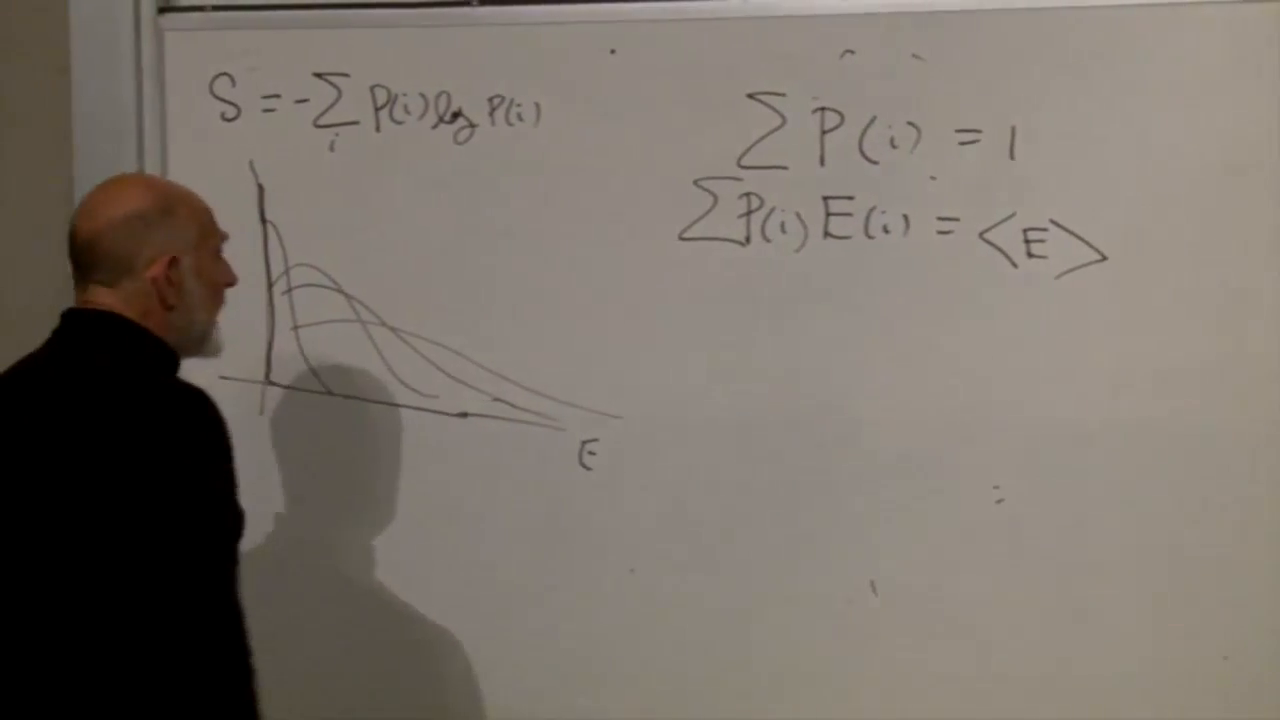
\includegraphics[width=0.88\textwidth]{lecture_03_figure_02.png}
\caption{На первой доске собраны формулы для энтропии, нормировки и средней энергии вместе с качественным семейством равновесных распределений.}
\lectureframe{00:06:44}
\end{figure}

\section{Равновесие как семейство распределений}

В предыдущей лекции у нас получилось однопараметрическое семейство равновесных распределений. Это семейство можно параметризовать температурой, но пока полезнее параметризовать его средней энергией \(\overline E\). При наименьшей возможной энергии распределение сосредоточено на основном состоянии:
\[
 P_i=\delta_{i0}.
\]
Тогда никакой неопределённости относительно состояния нет, и \(S=0\). По мере того как равновесное распределение распространяется на большее число энергетических уровней, растут и его средняя энергия, и его энтропия.

Это утверждение относится к тепловому семейству, а не ко всякому мыслимому распределению. Произвольное семейство могло бы смещаться к большим энергиям, одновременно сужаясь. Равновесные распределения, которые мы сейчас выведем, так себя не ведут в обычном режиме положительных температур. Вдоль этого семейства,
\begin{equation}
 \frac{dS}{d\overline E}>0.
 \label{eq:sm3-positive-temperature-branch}
\end{equation}
Системы с ограниченными спектрами могут также иметь ветви, на которых эта производная отрицательна. Такие режимы отрицательной температуры реальны, но в настоящем рассуждении мы их оставим в стороне.

Тепловое равновесие означает нечто большее, чем микроскопическую неподвижность. Молекулы продолжают двигаться, сталкиваться и обмениваться энергией. Стационарным стало макроскопическое описание: распределение больше не обнаруживает суммарного дрейфа, а отделённые части системы больше не поддерживают суммарный поток энергии.

\section{Законы термодинамики на языке статистики}

Первый закон — это закон сохранения энергии. Второй закон утверждает, что термодинамическая энтропия изолированной макроскопической системы не убывает:
\begin{equation}
 \Delta S_{\mathrm{tot}}\geq0.
 \label{eq:sm3-second-law}
\end{equation}
Равенство описывает равновесие или идеальное обратимое изменение; при спонтанной релаксации обычно имеет место строгое возрастание.

В вероятностной картине релаксация имеет тенденцию распределять вес по тем макроскопическим альтернативам, которые мы ещё различаем. Это утверждение требует оговорки, подчеркнутой на лекции: мы выполняем \emph{огрубление}. Точное гамильтоново развитие сохраняет тонкозернистую энтропию фазового пространства. Макроскопическая энтропия растёт потому, что мы перестаём отслеживать микроскопические корреляции и детали. Потеря такой информации расширяет редуцированное описание. Спонтанное сужение означало бы, напротив, что мы узнали микроскопическую информацию, не производя измерения.

Нулевой закон утверждает, что системы могут приходить к тепловому равновесию и что равновесие транзитивно. Если \(A\) находится в равновесии с \(B\), а \(B\) — с \(C\), то \(A\) находится в равновесии с \(C\). Температура задаёт величину, которая делает эту транзитивность наглядной:
\[
 T_A=T_B,\qquad T_B=T_C
 \quad\Longrightarrow\quad
 T_A=T_C.
\]
Вне равновесия энергия течёт от подсистемы с большей температурой к подсистеме с меньшей температурой. При равных температурах суммарный поток прекращается. Теперь мы выведем это операционное утверждение из энтропийного определения температуры.

\section{Почему энергия течёт от горячего к холодному}

Рассмотрим две слабо связанные подсистемы \(A\) и \(B\). Каждая из них находится во внутреннем равновесии, но их температуры различны. Выберем обозначения так, чтобы
\begin{equation}
 T_B>T_A>0.
 \label{eq:sm3-temperature-order}
\end{equation}
При малом обмене из сохранения полной энергии следует
\begin{equation}
 dE_A+dE_B=0.
 \label{eq:sm3-energy-conservation}
\end{equation}
Второй закон даёт
\begin{equation}
 dS_A+dS_B\geq0.
 \label{eq:sm3-entropy-change}
\end{equation}
Для каждой подсистемы, находящейся во внутреннем равновесии, температура определяется соотношением
\begin{equation}
 dE_X=T_X\,dS_X,
 \qquad X=A,B.
 \label{eq:sm3-temperature-differential}
\end{equation}
Подстановка в \eqref{eq:sm3-energy-conservation} даёт
\begin{equation}
 T_A\,dS_A+T_B\,dS_B=0,
\end{equation}
и, следовательно,
\begin{equation}
 dS_B=-\frac{T_A}{T_B}\,dS_A.
 \label{eq:sm3-dsb}
\end{equation}
Подставляя этот результат в \eqref{eq:sm3-entropy-change},
\begin{align}
 dS_{\mathrm{tot}}
 &=dS_A-\frac{T_A}{T_B}dS_A\\
 &=\frac{T_B-T_A}{T_B}\,dS_A\geq0.
 \label{eq:sm3-flow-entropy}
\end{align}
Поскольку \(T_B-T_A>0\) и \(T_B>0\), спонтанный обмен требует
\[
 dS_A>0.
\]
Тогда из \eqref{eq:sm3-temperature-differential} следует
\begin{equation}
 dE_A=T_A\,dS_A>0,
 \qquad
 dE_B=-dE_A<0.
 \label{eq:sm3-hot-to-cold}
\end{equation}
Энергия перетекла из \(B\), более горячей подсистемы, в \(A\), более холодную. Здесь теплота — это просто энергия в переносе. Поток продолжается до тех пор, пока не установится \(T_A=T_B\), когда изменение энтропии в первом порядке больше не благоприятствует ни одному направлению.

Тот же результат можно записать одной строкой:
\begin{equation}
 dS_{\mathrm{tot}}
 =dE_A\left(\frac{1}{T_A}-\frac{1}{T_B}\right)\geq0.
 \label{eq:sm3-compact-flow}
\end{equation}
Знак разности обратных температур определяет знак \(dE_A\). Эта компактная форма позднее естественно согласуется с каноническим ансамблем.

\begin{classroomqa}
\audiencequestion{Предполагает ли этот аргумент, что и \(A\), и \(B\) уже находятся во внутреннем равновесии?}
\lecturerresponse{Да. Приписывание одного \(T_A\) или \(T_B\) уже делает это предположение. Если подсистема не находится во внутреннем равновесии, разбейте её на меньшие области и применяйте этот аргумент локально везде, где можно определить температуру. Тогда глобальная релаксация складывается из обменов между этими областями.
\lecturetimestamp{00:24:38--00:25:22}}
\end{classroomqa}

\section{Что считать состоянием?}

Прежде чем искать равновесные вероятности, нужно понять, что означает метка \(i\). Микроскопическое состояние — это максимально полное описание системы, допускаемое лежащими в основе законами физики. В классической механике обычно мыслят положения и импульсы всех частиц. В квантовой механике состояние вместо этого представляет собой полное квантовое состояние; принцип неопределённости не позволяет одновременно точно задать все классические положения и импульсы.

Для квантовой системы в конечном ящике соответствующий счёт состояний может быть дискретным. Классическая статистическая механика возникает в подходящем пределе, где суммы по густо расположенным квантовым состояниям превращаются в интегралы по фазовому пространству. Этот предельный переход также вводит ячейку фазового пространства, необходимую для того, чтобы непрерывная энтропия была безразмерной; её нельзя получить простым заменением знака суммы на знак интеграла.

\begin{classroomqa}
\audiencequestion{Для газа следует ли представлять состояние как положения и импульсы каждой молекулы?}
\lecturerresponse{Это верная классическая картина. В более общем смысле состояние означает всё, что в принципе могло бы быть известно о системе, с учётом законов физики. Квантовая механика изменяет форму этого максимального описания и делает счёт при конечном объёме дискретным. Восстановление классического интеграла из квантовой суммы — это настоящий предельный переход, а не однострочная подстановка.
\lecturetimestamp{00:25:31--00:27:38}}
\end{classroomqa}

\section{Термостат из копий}

Теперь нельзя избежать трудного вопроса: после установления равновесия чем определяется \(P_i\)?

Поместим подсистему в контакт с очень большим термостатом. Энергия может переходить туда и обратно, но у термостата так много степеней свободы, что передача малого количества энергии почти не изменяет его температуру. Особенно удобный термостат состоит из многих слабо связанных копий самой подсистемы. Одна копия — это исследуемая система; остальные образуют её окружение.

Эта конструкция часто отражает реальную макроскопическую систему. Разделите большое почти однородное тело на много похожих ячеек. Каждая ячейка является подсистемой, а остальные ячейки служат для неё термостатом. Обозначим полное число копий через \(N\). В аудиторной демонстрации используются девять копий и три цветные метки состояний, но подсчёт не зависит от этих конкретных чисел.

Пусть \(n_i\) — число реплик в состоянии \(i\). Это \emph{числа заполнения}. Возможных энергетических уровней может быть бесконечно много, но при конечной полной энергии заполнение большинства очень высоких уровней пренебрежимо мало или равно нулю.

Первое ограничение — это просто число реплик:
\begin{equation}
 \sum_i n_i=N.
 \label{eq:sm3-number-constraint}
\end{equation}
Второе — полная энергия:
\begin{equation}
 \sum_i n_iE_i=N\overline E.
 \label{eq:sm3-total-energy-constraint}
\end{equation}
Правая часть экстенсивна. Если число реплик удвоить, удерживая их статистическое состояние фиксированным, полная энергия удваивается, тогда как средняя энергия на реплику остаётся \(\overline E\).

\begin{classroomqa}
\audiencequestion{Должно ли построение из реплик также удовлетворять энергетическому ограничению?}
\lecturerresponse{Да. Числа заполнения должны суммироваться в \(N\), а их взвешенная по энергии сумма должна равняться фиксированной полной энергии \(N\overline E\). Это как раз те два ограничения, которые позже будут наложены при максимизации энтропии.
\lecturetimestamp{00:37:12--00:39:54}}
\end{classroomqa}

Вероятность того, что случайно выбранная реплика находится в состоянии \(i\), равна её относительной частоте:
\begin{equation}
 P_i=\frac{n_i}{N},
 \qquad
 n_i=NP_i.
 \label{eq:sm3-frequency-probability}
\end{equation}

\begin{figure}[t]
\centering
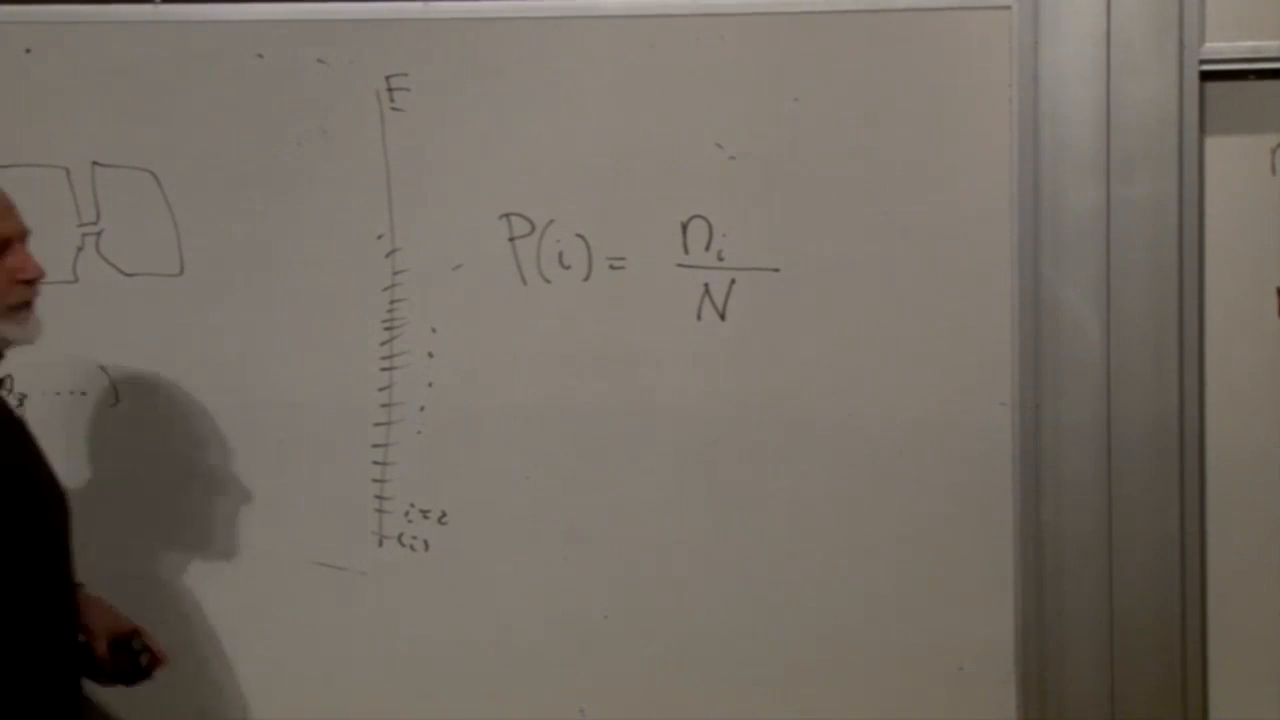
\includegraphics[width=0.82\textwidth]{lecture_03_figure_03.png}
\caption{Картина энергетических уровней и отождествление вероятности с долей заполнения \(P_i=n_i/N\).}
\lectureframe{00:41:40}
\end{figure}

\begin{classroomqa}
\audiencequestion{Означает ли запись \(N(i)\) на доске нечто отличное от \(n_i\)?}
\lecturerresponse{Нет. Оба обозначения означают число заполнения состояния \(i\). Мы последовательно используем \(n_i\), а прописную \(N\) оставляем для полного числа реплик.
\lecturetimestamp{00:41:28--00:41:33}}
\end{classroomqa}

Разделив \eqref{eq:sm3-number-constraint} и
\eqref{eq:sm3-total-energy-constraint} на \(N\), мы вновь получаем ограничения на вероятности:
\begin{equation}
 \sum_iP_i=1,
 \qquad
 \sum_iP_iE_i=\overline E.
 \label{eq:sm3-probability-constraints}
\end{equation}
Таким образом, частотная интерпретация ансамбля воспроизводит уравнения, с которых мы начали.

\section{Кратность схемы заполнения}

Зафиксируем набор чисел заполнения \(\{n_i\}\). Сколькими способами можно распределить \(N\) различимых реплик по состояниям так, чтобы реализовался в точности этот набор? Ответ даётся мультиномиальным коэффициентом
\begin{equation}
 C(\{n_i\})=\frac{N!}{\prod_i n_i!}.
 \label{eq:sm3-multiplicity}
\end{equation}
Чтобы понять знаменатель, сначала расположим все \(N\) помеченные реплики в \(N!\) порядках. Перестановка \(n_i\) реплик, занимающих одно и то же состояние, не даёт нового распределения реплик по состояниям, поэтому для каждого состояния нужно делить на \(n_i!\).

\begin{figure}[t]
\centering
\includegraphics[width=0.88\textwidth]{lecture_03_figure_04.png}
\caption{Мультиномиальная кратность
\(C=N!/\prod_i n_i!\), записанная на доске.}
\lectureframe{00:46:55}
\end{figure}

Незаполненные уровни не создают проблемы, поскольку \(0!=1\). Если все реплики занимают одно состояние, то
\[
 C=\frac{N!}{N!}=1,
\]
как и следует ожидать. Если три реплики занимают три различные заданные состояния, то
\[
 C=\frac{3!}{1!\,1!\,1!}=6.
\]
Если две реплики занимают два заданных состояния, формула даёт два распределения: можно поменять местами, какая помеченная реплика какое состояние занимает.

\begin{classroomqa}
\audiencequestion{Может ли более чем один набор чисел заполнения удовлетворять двум ограничениям?}
\lecturerresponse{Обычно таких наборов много. Уравнение
\eqref{eq:sm3-multiplicity} сначала подсчитывает число распределений для одного фиксированного набора
\(\{n_i\}\), ещё не решая, удовлетворяет ли он ограничениям. На следующем этапе сравниваются все наборы, совместимые с ограничениями, и находится тот, у которого кратность наибольшая.
\lecturetimestamp{00:48:07--00:48:43}}
\end{classroomqa}

Статистическое предположение состоит в том, что микроскопические распределения, совместимые с изолированными условиями, рассматриваются симметрично. Поэтому макроскопическая схема заполнения, реализуемая большим числом распределений, более вероятна. При больших
\(N\) распределение по долям \(n_i/N\) становится резко заострённым.
Равновесные доли — это значения, максимизирующие \(C\) при условиях
\eqref{eq:sm3-number-constraint} и
\eqref{eq:sm3-total-energy-constraint}.

\section{Приближение Стирлинга}

Факториалы становятся огромными задолго до того, как \(N\) достигает макроскопического значения, поэтому мы работаем с их логарифмами. Начнём с
\begin{equation}
 \log N!=\sum_{x=1}^{N}\log x.
 \label{eq:sm3-log-factorial-sum}
\end{equation}
Для больших \(N\) сумма приближается площадью под \(\log x\):
\begin{align}
 \log N!
 &\simeq\int_1^N\log x\,dx\\
 &=\left[x\log x-x\right]_1^N\\
 &=N\log N-N+1.
 \label{eq:sm3-stirling-integral}
\end{align}
Первообразная непосредственно следует из
\[
 \frac{d}{dx}(x\log x-x)=\log x.
\]
В ведущем экстенсивном порядке аддитивную константу можно отбросить:
\begin{equation}
 \log N!\simeq N\log N-N.
 \label{eq:sm3-stirling-log}
\end{equation}
Возведение в экспоненту даёт упрощённую форму, использованную в лекции,
\begin{equation}
 N!\simeq N^N e^{-N}.
 \label{eq:sm3-stirling-simple}
\end{equation}

\begin{figure}[t]
\centering
\includegraphics[width=0.88\textwidth]{lecture_03_figure_05.png}
\caption{Старшее приближение Стирлинга и его вывод заменой суммы \(\log x\) интегралом.}
\lectureframe{01:03:45}
\end{figure}

\begin{classroomqa}
\audiencequestion{Не остаётся ли при вычислении \(x\log x-x\) на нижнем пределе дополнительное \(+1\)?}
\lecturerresponse{Да. Уравнение \eqref{eq:sm3-stirling-integral} содержит эту константу. Она пренебрежимо мала по сравнению с членами, пропорциональными \(N\), при \(N\to\infty\), поэтому в ведущей формуле её опускают. Сама сумма должна начинаться с \(x=1\); \(\log0\) не определён.
\lecturetimestamp{01:04:12--01:04:35}}
\end{classroomqa}

\begin{classroomqa}
\audiencequestion{Не отсутствует ли также множитель, пропорциональный \(\sqrt{N}\)?}
\lecturerresponse{Да. Более точная асимптотическая формула имеет вид
\[
 N!\sim\sqrt{2\pi N}\left(\frac{N}{e}\right)^N.
\]
Её логарифм добавляет лишь \(\tfrac12\log(2\pi N)\), что субэкстенсивно по сравнению с \(N\log N-N\). Это важно для точных вероятностей при конечном \(N\), но не для ведущего расчёта энтропии макроскопической системы.
\lecturetimestamp{01:04:35--01:05:40}}
\end{classroomqa}

Приближение Стирлинга нужно также применять с осторожностью в знаменателе
\eqref{eq:sm3-multiplicity}. В термодинамическом пределе состояния с ненулевыми предельными вероятностями имеют \(n_i=NP_i\), так что их заполнения растут вместе с \(N\). Состояния с очень малым или исчезающим заполнением можно обработать, введя отсечение по конечной энергии, а затем восстановить предельным переходом. Ведущая экстенсивная энтропия не зависит от отброшенных подведущих членов.

\section{Логарифм кратности — это энтропия}

Применим \eqref{eq:sm3-stirling-simple} к числителю и ко всем макроскопически заполненным множителям в знаменателе:
\begin{equation}
 C\simeq
 \frac{N^Ne^{-N}}
 {\prod_i n_i^{\,n_i}e^{-n_i}}.
 \label{eq:sm3-c-stirling}
\end{equation}
Поскольку \(\sum_i n_i=N\), ведущие экспоненциальные множители сокращаются:
\begin{equation}
 C\simeq\frac{N^N}{\prod_i n_i^{\,n_i}}.
 \label{eq:sm3-c-leading}
\end{equation}
Максимизировать логарифм легче, чем произведение, а логарифм монотонен, поэтому оба максимума достигаются при одной и той же схеме заполнения:
\begin{equation}
 \log C=N\log N-\sum_i n_i\log n_i.
 \label{eq:sm3-logc-occupations}
\end{equation}
Теперь подставим \(n_i=NP_i\):
\begin{align}
 \log C
 &=N\log N-\sum_iNP_i\log(NP_i)\\
 &=N\log N-N\sum_iP_i\log N
   -N\sum_iP_i\log P_i\\
 &=-N\sum_iP_i\log P_i,
 \label{eq:sm3-logc-entropy-derivation}
\end{align}
где благодаря нормировке сокращаются два члена \(N\log N\). Следовательно, в ведущем порядке по \(N\),
\begin{equation}
 \boxed{\log C=NS}.
 \label{eq:sm3-logc-ns}
\end{equation}

\begin{figure}[t]
\centering
\includegraphics[width=0.88\textwidth]{lecture_03_figure_06.png}
\caption{Вычисление на доске, связывающее
\(\log C=N\log N-\sum_i n_i\log n_i\) с
\(-N\sum_iP_i\log P_i=NS\).}
\lectureframe{01:16:10}
\end{figure}

Это соотношение — идейный центр главы. Энтропия не является посторонней величиной, навязанной задаче подсчёта. Это логарифм кратности, отнесённый к одной реплике. Поэтому максимизация числа микроскопических распределений тождественна, в ведущем порядке, максимизации энтропии одной реплики.

\begin{classroomqa}
\audiencequestion{Разве кратность не была бы наибольшей, если бы все числа заполнения были равны?}
\lecturerresponse{Равномерное распределение получается, когда никакое состояние не выделено и на конечном наборе состояний наложено только
\(\sum_i n_i=N\). Ограничение фиксированной энергии меняет ответ, потому что значения \(E_i\) различны. Равные заполнения, вообще говоря, не дают заданной средней энергии.
\lecturetimestamp{01:17:07--01:18:20}}
\end{classroomqa}

\begin{classroomqa}
\audiencequestion{Величина \(N\) велика, но почему приближение Стирлинга можно применять к каждому \(n_i\) в знаменателе?}
\lecturerresponse{Для каждого состояния с ненулевой предельной вероятностью
\(n_i=NP_i\) растёт пропорционально \(N\). Можно сначала сохранить конечный энергетический диапазон, взять в нём предел при больших \(N\), а затем расширить этот диапазон. Разреженные хвостовые состояния требуют отдельных конечных поправок, но они не изменяют ведущую экстенсивную энтропию.
\lecturetimestamp{01:18:23--01:19:28}}
\end{classroomqa}

\begin{classroomqa}
\audiencequestion{Именно это приближение при больших \(N\) ранее имелось в виду под огрублением?}
\lecturerresponse{Нет. Термодинамический предел управляет большими числами заполнения и асимптотическим подсчётом. Огрубление — это потеря или намеренное отбрасывание микроскопического разрешения. Это разные операции, хотя обе часто используются в макроскопической статистической механике.
\lecturetimestamp{01:19:29--01:19:46}}
\end{classroomqa}

\begin{classroomqa}
\audiencequestion{Поскольку
\(\log C=N\log N-\sum_i n_i\log n_i\), не следует ли минимизировать второй член, а не максимизировать его?}
\lecturerresponse{Да; при фиксированном \(N\) максимизация \(\log C\) эквивалентна минимизации \(\sum_i n_i\log n_i\). После подстановки \(n_i=NP_i\) фиксированные члены \(N\log N\) сокращаются, и остаётся
\(-N\sum_iP_i\log P_i=NS\). Тем самым ту же самую операцию естественнее описывать как максимизацию положительной энтропии \(S\).
\lecturetimestamp{01:19:48--01:20:55}}
\end{classroomqa}

\begin{classroomqa}
\audiencequestion{Почему не завершить рассуждение сразу по соображениям симметрии и не положить все \(n_i\) равными?}
\lecturerresponse{Этот короткий путь игнорирует энергетические метки. Ограничение нормировки трактует состояния симметрично, но
\(\sum_iP_iE_i=\overline E\) этого не делает: состояния с разной энергией вносят разный вклад. Именно в энергетическом ограничении и появляется неравномерное равновесное распределение.
\lecturetimestamp{01:21:15--01:21:41}}
\end{classroomqa}

\section{Задача максимизации энтропии}

Теперь мы можем сформулировать статистико-механическое правило без двусмысленности. Варьируйте вероятности \(P_i\) и максимизируйте
\begin{equation}
 S[P]=-\sum_iP_i\log P_i
 \label{eq:sm3-maximize-entropy}
\end{equation}
при условиях
\begin{equation}
 \sum_iP_i=1,
 \qquad
 \sum_iP_iE_i=\overline E.
 \label{eq:sm3-maxent-constraints}
\end{equation}
Вероятности, при которых достигается максимум, задают резко предпочтительные доли заполнения в большом ансамбле реплик. Числа заполнения флуктуируют, но их относительные отклонения уменьшаются с ростом \(N\), так что отношения \(n_i/N\) становятся хорошо определёнными термодинамическими вероятностями.

\begin{classroomqa}
\audiencequestion{Являются ли \(E_i\) фиксированными энергиями состояний, тогда как в ограничении используется отдельно заданная полная энергия?}
\lecturerresponse{Да. Спектр \(\{E_i\}\) относится к подсистеме.
Полная совокупность реплик имеет фиксированную полную энергию, но энергия
непрерывно переходит между репликами. Деление этой полной энергии на \(N\) фиксирует среднюю
энергию \(\overline E\) одной реплики, а не её энергию в каждой микроскопической
реализации.
\lecturetimestamp{01:26:12--01:27:07}}
\end{classroomqa}

Задачу легко сформулировать, но она ещё не решена. Это задача на экстремум с двумя ограничениями, поэтому нужен ещё один математический инструмент.

\section{Множители Лагранжа}

Для функции \(F(x_1,x_2,\ldots)\) без ограничений стационарная точка
удовлетворяет
\begin{equation}
 \frac{\partial F}{\partial x_i}=0
 \qquad\text{for every }i.
 \label{eq:sm3-unconstrained-stationary}
\end{equation}
Теперь потребуем дополнительно, чтобы
\begin{equation}
 G(x_1,x_2,\ldots)=0.
 \label{eq:sm3-one-constraint}
\end{equation}

\begin{classroomqa}
\audiencequestion{Что означает \(x\), если на рисунке координатами служат \(x\)
и \(y\)?}
\lecturerresponse{Здесь \(x\) — сокращённое обозначение всего вектора координат
\((x_1,x_2,\ldots)\). На двумерном рисунке его компонентами являются
просто \(x\) и \(y\). Позже компонентами будут вероятности
\(P_1,P_2,\ldots\).
\lecturetimestamp{01:30:12--01:30:20}}
\end{classroomqa}

Геометрически линии уровня \(F=\text{constant}\) образуют контурную карту,
а \(G=0\) — кривую, по которой системе разрешено двигаться. Условный
экстремум возникает там, где одна из линий уровня \(F\) касается кривой
ограничения. В этой точке градиенты параллельны:
\begin{equation}
 \nabla F=-\lambda\nabla G
 \label{eq:sm3-parallel-gradients}
\end{equation}
для некоторого числа \(\lambda\).

\begin{figure}[t]
\centering
\includegraphics[width=0.88\textwidth]{lecture_03_figure_07.png}
\caption{Геометрия линий уровня на доске и дополненная функция
\(F'=F+\lambda G\). Условный экстремум возникает в точке касания.}
\lectureframe{01:37:10}
\end{figure}

Уравнение \eqref{eq:sm3-parallel-gradients} можно получить, определив
дополненную функцию
\begin{equation}
 F'=F+\lambda G
 \label{eq:sm3-augmented-function}
\end{equation}
и потребовав обычной стационарности:
\begin{equation}
 \frac{\partial F'}{\partial x_i}=0.
 \label{eq:sm3-augmented-stationarity}
\end{equation}
Множитель \(\lambda\) поначалу неизвестен. Из-за этого система не
остаётся недоопределённой, потому что исходное ограничение \(G=0\) даёт ещё
одно уравнение.

\begin{classroomqa}
\classquestion{Почему добавление члена, пропорционального \(G\), делает
стационарной точку, удовлетворяющую ограничению?}
\lecturerresponse{В условном экстремуме смещение по касательной к \(G=0\)
уже не даёт изменения \(F\) в первом порядке. Остаётся только наклон по
нормали к ограничению. Поскольку \(\nabla G\) направлен в ту же нормальную
сторону, подходящий \(\lambda\) его компенсирует:
\(\nabla F+\lambda\nabla G=0\).
\lecturetimestamp{01:35:06--01:35:32}}
\end{classroomqa}

\section{Пример с двумя переменными}

Требуется минимизировать
\begin{equation}
 F(x,y)=\frac{x^2+y^2}{2}
 \label{eq:sm3-example-f}
\end{equation}
при условии
\begin{equation}
 x+y=1.
 \label{eq:sm3-example-constraint}
\end{equation}
Запишем ограничение как \(G=x+y-1=0\) и составим
\begin{equation}
 F'=\frac{x^2+y^2}{2}+\lambda(x+y-1).
 \label{eq:sm3-example-augmented}
\end{equation}
Стационарные уравнения имеют вид
\begin{align}
 \frac{\partial F'}{\partial x}&=x+\lambda=0,\\
 \frac{\partial F'}{\partial y}&=y+\lambda=0.
 \label{eq:sm3-example-derivatives}
\end{align}
Следовательно, \(x=y=-\lambda\). Оставшееся уравнение — это ограничение,
\[
 x+y=-2\lambda=1,
\]
поэтому
\begin{equation}
 \lambda=-\frac12,
 \qquad
 x=y=\frac12.
 \label{eq:sm3-example-solution}
\end{equation}
Точка \((1/2,1/2)\) — это место, где наименьшая окружность с центром в начале
координат касается прямой \(x+y=1\).

\begin{figure}[t]
\centering
\includegraphics[width=0.88\textwidth]{lecture_03_figure_08.png}
\caption{Полное вычисление методом множителей Лагранжа для минимизации
\((x^2+y^2)/2\) при условии \(x+y=1\).}
\lectureframe{01:44:10}
\end{figure}

При нескольких ограничениях введите по одному множителю для каждого:
\begin{equation}
 F'=F+\lambda_1G_1+\lambda_2G_2+\cdots.
 \label{eq:sm3-many-multipliers}
\end{equation}
Затем решайте
\begin{equation}
 \begin{aligned}
 \frac{\partial F'}{\partial x_i}&=0
 &&\text{for every }i,\\
 G_a&=0
 &&\text{for every constraint }a.
 \end{aligned}
 \label{eq:sm3-many-equations}
\end{equation}
В лекции предлагается намеренно искусственная тренировочная задача: найти
экстремум квадратичной функции от \(x,y,z\) при наложении двух независимых
линейных ограничений, например \(x+y=1\) и \(z+x=1\). Её цель — не конкретный
ответ, а правило, что каждое ограничение вносит и один множитель, и одно
уравнение.

\section{Задача, подготовленная к следующей лекции}

В статистической механике координатами служат вероятности
\(\{P_i\}\), максимизируемой функцией является энтропия, а ограничениями
— нормировка и фиксированная средняя энергия. Определим
\begin{align}
 S[P]&=-\sum_iP_i\log P_i,\\
 G_1[P]&=\sum_iP_i-1,\\
 G_2[P]&=\sum_iP_iE_i-\overline E.
 \label{eq:sm3-final-functions}
\end{align}
Поэтому дополненную энтропию можно записать в виде
\begin{equation}
 \Phi[P]
 =S[P]+\alpha G_1[P]+\beta G_2[P].
 \label{eq:sm3-final-augmented}
\end{equation}
Уравнения, которые нужно решить, таковы:
\begin{equation}
 \frac{\partial\Phi}{\partial P_i}=0
 \quad\text{for every }i,
 \qquad
 G_1=0,
 \qquad
 G_2=0.
 \label{eq:sm3-final-problem}
\end{equation}

\begin{figure}[H]
\centering
\includegraphics[width=0.88\textwidth]{lecture_03_figure_09.png}
\caption{Заключительная запись на доске: энтропия как функция вероятностей
вместе с нормировкой и фиксированной средней энергией.}
\lectureframe{01:53:05}
\end{figure}

На этом этапе задача полностью поставлена. Решение
\eqref{eq:sm3-final-problem} даёт равновесное распределение. Множитель,
сопряжённый с энергией, станет обратной температурой
\(\beta=1/T\) с точностью до соглашения о знаке, выбранного в
\eqref{eq:sm3-final-augmented}. На следующей лекции выполняется это
дифференцирование и получаются больцмановские веса.
